\documentclass[12pt]{amsart}
\usepackage[margin = 1in]{geometry}
\usepackage{amsmath, amssymb, amsthm, graphicx}
\usepackage{enumerate}
\usepackage[all]{xy}
\usepackage{mathrsfs}

%%%%%%%%%%%%%% COLOR COMMENTS! %%%%%%%%%%%%%%%
\usepackage{color}
\newcommand{\dzb}[1]{{\color{blue} \sf
    $\spadesuit\spadesuit\spadesuit$ DZB: [#1]}}
\newcommand{\reword}[1]{{\color{red} \sf $\spadesuit\spadesuit\spadesuit$ reword: [#1]}}

% changed above definition to make comments disappear
%\newcommand{dzb}[1]{}
%\newcommand{reword}[1]{}

% Color names: http://en.wikibooks.org/wiki/LaTeX/Colors#The_68_standard_colors_known_to_dvips
\usepackage[usenames,dvipsnames]{xcolor}
\newcommand{\note}[1]{{\color{BurntOrange} $\blacktriangle\blacktriangle$\sf Note: [#1]}}

\newcommand{\F}[0]{\mathbb{F}}
\newcommand{\tr}[0]{\operatorname{tr}}
\newcommand{\wt}[1]{\widetilde{#1}}
\newcommand{\frob}[0]{\operatorname{Frob}}
\newcommand{\card}[0]{\#}
\newcommand{\pmat}[4]{\begin{pmatrix}#1 & #2 \\ #3 & #4\end{pmatrix}}
\newcommand{\pderiv}[2]{\frac{\partial #1}{\partial #2}}
\newcommand{\Ov}{\mathcal{O}_{v}}
\newcommand{\Ok}{\mathcal{O}_{K}}
\newcommand{\Q}{\mathbb{Q}}
\newcommand{\Z}{\mathbb{Z}}
\newcommand{\C}{\mathbb{C}}
\newcommand{\leg}[2]{\left(\frac{#1}{#2}\right)}
\newcommand{\calO}{\mathcal{O}}
\newcommand{\frakp}{\mathfrak{p}}
\newcommand{\frakq}{\mathfrak{q}}
\newcommand{\mf}[1]{\mathfrak{#1}}
\newcommand{\nm}{\operatorname{N}_{K/\Q}}
\newcommand{\Cl}{\operatorname{Cl}}
\newcommand{\oo}{\mathcal{O}}
\newcommand{\sgn}{\operatorname{sgn}}
\newcommand{\Gal}{\operatorname{Gal}}
\newcommand{\cl}{\overline}
\newcommand{\mc}[1]{\mathcal{#1}}
\newcommand{\Cc}{\mathcal{C}}
\newcommand{\Dc}{\mathcal{D}}
\newcommand{\raym}{\mathcal{C}^{\frakm}_K}
\newcommand{\frakr}{\mathfrak{r}}
\newcommand{\Spec}{\text{Spec} \ }
\newcommand{\Hom}{\text{Hom}}
\newcommand{\ord}{\text{ord}}
\newcommand{\scr}[1]{\mathscr{#1}}
\newcommand{\R}{\mathbb{R}}
\newcommand{\cal}[1]{\mathcal{#1}}
\newcommand{\Nm}{\text{Nm}}
\newcommand{\A}{\mathbb{A}}
\newcommand{\ti}{\times}
\newcommand{\Hbb}{\mathbb{H}}
%\newcommand{\leg}[2]{\left(\frac{ \# 1}{\# 2} \right)}

\DeclareMathOperator{\GL}{GL}
\DeclareMathOperator{\SL}{SL}
\DeclareMathOperator{\Frob}{Frob}
\DeclareMathOperator{\ab}{ab}
\DeclareMathOperator{\cyc}{cyc}
\DeclareMathOperator{\N}{N}
\DeclareMathOperator{\Ver}{Ver}
\DeclareMathOperator{\Art}{Art}
\DeclareMathOperator{\Spl}{Spl}
\DeclareMathOperator{\sep}{sep}
\DeclareMathOperator{\Stab}{Stab}
\DeclareMathOperator{\Sp}{Sp}
\DeclareMathOperator{\SO}{SO}
\DeclareMathOperator{\SU}{SU}
\DeclareMathOperator{\PGL}{PGL}
\DeclareMathOperator{\Mat}{Mat}
\DeclareMathOperator{\Tr}{Tr}
\DeclareMathOperator{\End}{End}
\DeclareMathOperator{\Ad}{Ad}
\DeclareMathOperator{\Aut}{Aut}
\DeclareMathOperator{\WPr}{WPr}

\newtheorem{thm}{Theorem}
\newtheorem{lemma}[thm]{Lemma}
\newtheorem{defn}[thm]{Definition}
\newtheorem{prop}[thm]{Proposition}
\newtheorem{cor}[thm]{Corollary}
\newtheorem{ex}[thm]{Example}
\newtheorem{crit}[thm]{Criterion}


\theoremstyle{remark}
\newtheorem{rem}[thm]{Remark}

\makeatletter
\def\imod#1{\allowbreak\mkern5mu({\operator@font mod}\,\,#1)}
\makeatother

\widowpenalty=1000
\clubpenalty=1000

\title{CS 181 Problem Set 2}
\author{Ashok Cutkosky and Tony Feng}


\begin{document}
\maketitle

\noindent \textbf{Problem 1.}



\noindent \textbf{Problem 2.}

\noindent \textbf{Problem 3.}

\begin{itemize}
\item[1.-4.] See source code.

\item[5.]

\item[6.]
\begin{itemize}
\item[a.] Learning rate 0.05
\item[b.] 

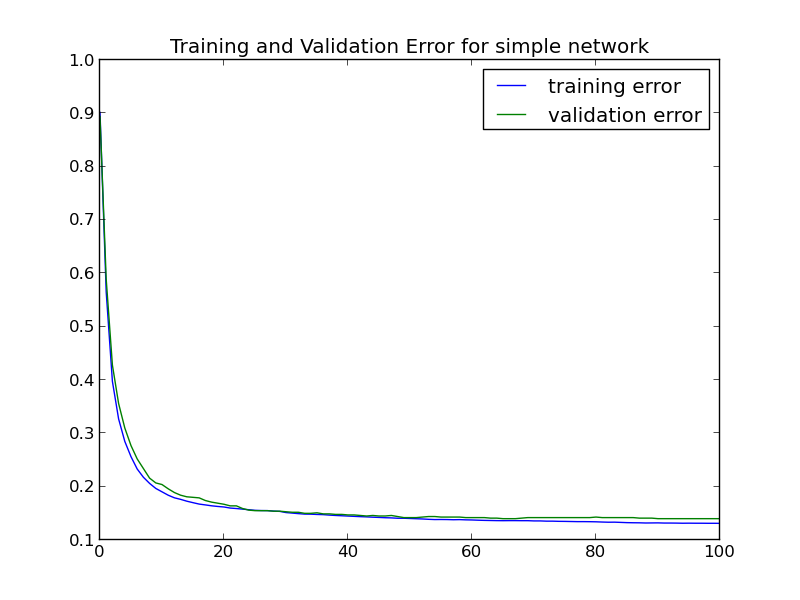
\includegraphics[height =2in]{simple100_005}

60 is a good number of epochs to train for, since validation set error stops decreasing at that point. It is important to use the validation set to tune the number of epochs because the validation set will measure how well our learning on the test set generalizes to other examples, so that we avoid overfitting.

\item[c.] At 60 epochs the training set performance was 0.863 and the validation set performance was 0.858.

\end{itemize}

\end{itemize}
\noindent \textbf{Problem 4.}

\begin{itemize}

\item[1.]
$C$ is attempting to address the complexity of the network - it is implementing regularization. A network in which many weights are actually zero represents a graph in which some nodes in one layer are actually not connected to nodes in the next layer, which is a simpler scenario than the fully-connected network. The additional summation in $C$ penalizes higher weights so that the network will limit its complexity.

\item[2.]
If our learning rate is $\alpha$, then we want the update rule to be 
\[
{w_{{mj}}}^{r+1}\from {w_{mj}}^r + \alpha \frac{\del C}{\del w_{mj}}
\]
Now we have
\[
C=\mathcal{L}+\lambda \sum {w_{mj}}^2
\]
Where the second sum runs over all the weights in the network.
Thus
\[
\frac{\del C}{\del w_{mj}} = \frac{\del \mathcal{L}}{\del w_{mj}}+2\lambda w_{mj}
\]
We already know $\frac{\del \mathcal{L}}{\del w_i}$ from the original backprogagation rule. Thus our update rule is
\[
{w_{mj}}^{r+1}\from {w_{mj}^{r}+\alpha a_{m}\delta_j-2\alpha\lambda w_{mj}
\]
\end{itemize}


\end{document}



